\chapter{前言}
\section{应用背景:协同编辑应用}
	\par 协同编辑系统,可以允许不同地点的用户同时编辑同一份文档。为了获得较快的响应和较高的实用性,系统会在不同的地点或设备进行文档的复制。一个用户可以在某个副本上进行文档的编辑,并将做出的修改异步地传递给其他副本。不必要等待服务器处理完再响应用户操作,本地操作可以立即执行。同时系统必须保证编辑的一致性,即在所有用户完成文档的编辑后,所有的副本内容一致。

\section{技术背景:Replicated List 规约及其基于OT的 Replicated List 算法}

\subsection{规约}
List 支持的常见简单操作 (insert, del, read)

规约: convergence (strong eventual consistency)
Def2 and Def3 of ``SSS''

SIGMOD89 Page 4

\subsection{OT}
Operational Transformation(OT)是一种为了支持协作功能,在协作软件系统中所采用的技术。OT最早在1989年被提出,是为了在纯文本文档的协同编辑中实现一致性和并发控制所发明的,经过二十余年的研究,OT的能力已经得到了拓展,在2009年OT做为一种核心技术被Apache Wave和Google Docs所采用来实现其合作特点。
OT的基本思想是根据先前执行的并发操作的影响,对正在编辑的操作的参数进行转换或调整,是转换后的操作能够达到正确地操作,并且保持文档的一致性。
\section{OT-based 协议}
client-server 结构

一个OT系统包含2个关键的部分,上层的控制算法和底层的OT函数。
\begin{figure}[H]
\centering
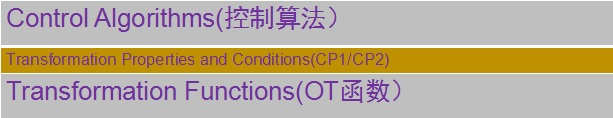
\includegraphics{figures/OT structure.jpg}
\caption{OT系统结构}
\end{figure}

控制算法负责决定哪些操作以何种顺序进行转换,而具体的OT函数则实施具体的两个操作之间的变化。
OT函数的数量由OT系统的模型所支持的数据和操作类型所决定。
这两者由一系列转换条件和属性结合在一起,所以整个OT系统的正确性就是由控制算法和OT函数的正确性以及协议的正确性所共同决定的。

由于这种分层结构,我们可以单独考虑OT函数的设计,而不必关心控制算法。

\section{本文研究工作: 面向 Redis List的OT函数的设计与验证}
	\par 本次毕业设计的目标是实现Redis List所支持的14种非阻塞操作的OT(Operational Transformation)函数,并且对实现函数的正确性进行验证。阿里云和RedisLab的团队目前都在对Redis List的操作进行开发,Redis List操作的OT函数实现具有应用前景和商业前途。

	\par 在OT函数的设计方面,本文使用数学公式表示出所有OT函数的基本形式,并且绘制图片和表格进行相应说明。

	\par 在OT函数的验证方面,使用TLA +完成了对所设计OT函数的验证,证明其满足CP1正确性,并且对验证代码的复杂度进行了相应分析。
\section{论文组织}
	\par 本文后续内容组织如下:
	\par 第2章介绍本文的相关工作,包括系统模型和已有的相关OT函数的设计。
	\par 第3章介绍了Redis列表相关的基本命令,并对其进行了分类,然后进行了对应OT函数的设计。
	\par 第4章介绍了TLA+,并使用TLA+完成了对上述设计好的OT函数的验证,对实验结果进行了分析
	\par 第5章是本论文的结论和以后工作的相关展望。